\documentclass[a4paper,10pt]{scrartcl}
\usepackage[utf8]{inputenc}
\usepackage{hyperref}
\usepackage{graphicx}
\graphicspath{ {./images/} }


\usepackage{float}


\title{Server Set-Up \& Security-Hardening Script 2.0}
\author{Anna Albrecht and Samuel Imboden}

\subtitle {Manual}


\begin{document}

\maketitle


\pagebreak
\tableofcontents
\pagebreak

\section{Introduction}

The purpose of the Server Set-Up \& Security-Hardening Script 2.0 is to help the user to set up an internet server easily and independently. This project was created by us as a project 1 for our computer science studies at the Bern University of Applied Science (BFH). It is based on the Server Set-Up \& Security-Hardening Script 1.0 which can be fond on \url{https://github.com/SSSHS}.

\subsection{Prerequisites}
Before you will be able to run the script properly you need to have the following things ready:

\subsubsection{Ubuntu 20.04 Server}

You will need root access to a Server with Ubuntu 20.04 running. You can get a virtual private server (VPS) from \url{https://us.ovhcloud.com} or from any other provider such as Amazon. \newline

\noindent If you already have a server with Ubuntu 18.04 an upgrade will be needed first. You can do so by using the following command: sudo do-release-upgrade -d . Note that this may take several minutes.

\subsubsection{Domain(s)}

To make use of the web server or mail server you will need at least one domain. It is possible to set up multiple domains on your web and mail server. \newline

\noindent Please remember to set your domain to the IP-address of your server. This can usually be done on the website of your domain provider. Note that it may take several hours until the change is effective.

\subsubsection{Minimal Linux knowledge}

You will need minimal knowledge of the Linux command line, as you need to clone the Github repository, run the script and move some files.

\pagebreak


\subsection{Differences to SSSHS 1.0}

In version 1.0 of the SSSHS all components were installed directly to the Ubuntu Server. \newline

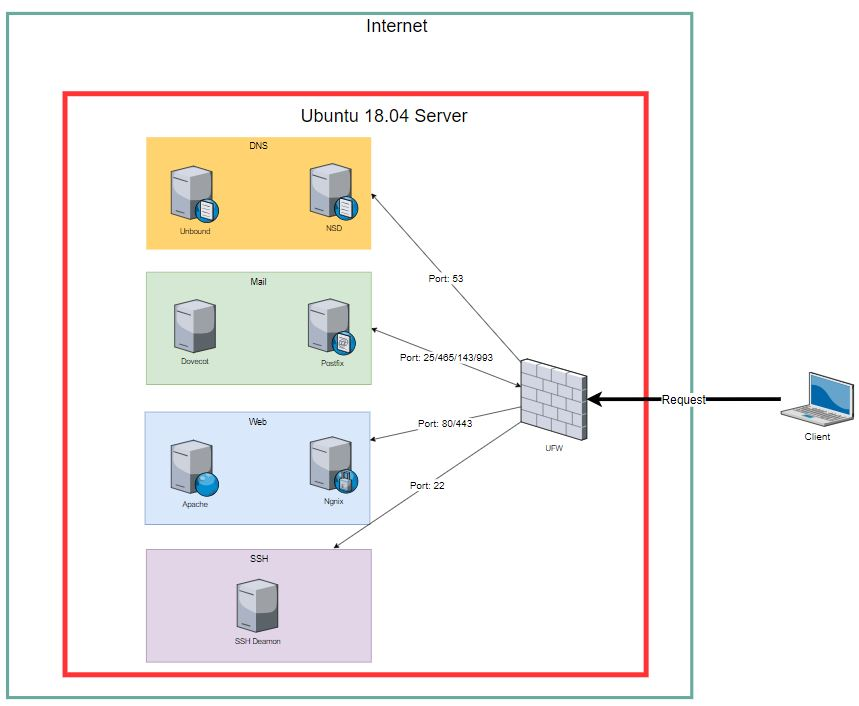
\includegraphics[width=\textwidth]{overview}

\pagebreak

\noindent In version 2.0 many components are running inside Docker containers for better security and control. There is also an intrusion detection that will log suspicious packets. There is now the possibility to set up a Jitsi Server or a Tor relay. The mail server has been changed to Mail in a Box, which already comes with many useful components and a web interface. There is also the possibility to run a database (sql or nosql) in a Docker container. If you prefer an more simple installation without Docker, please use the version 1.0 of the SSSHS. \newline

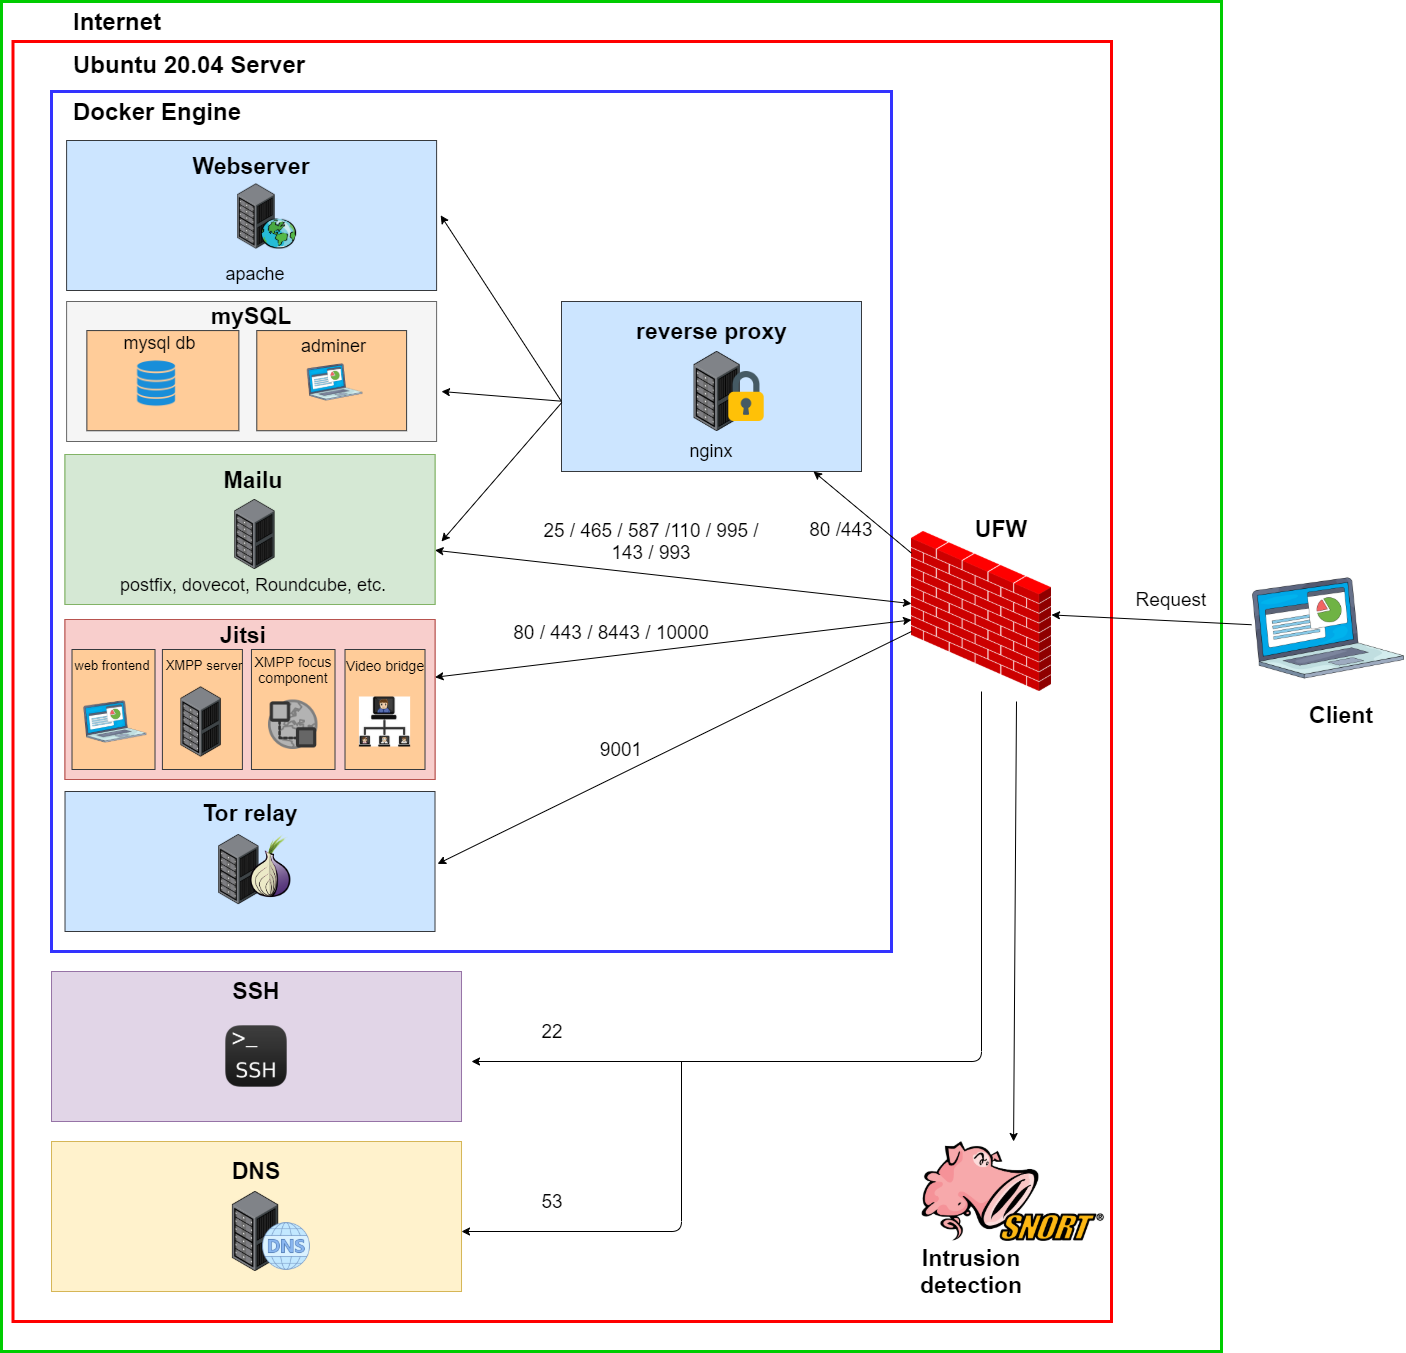
\includegraphics[width=\textwidth]{overview2}

\pagebreak

\section{Manual}

As a first step clone the Github repository form \url{https://github.com/SSSHS-2-0/script.git}

\noindent After cloning the repository from Github, run the "setup.sh" script in the main directory(script). You will see the following graphical interface: \newline

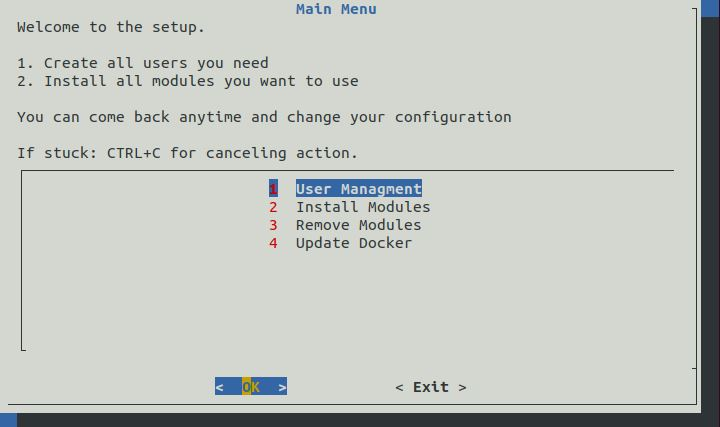
\includegraphics[width=\textwidth]{mainmenu} \newline


\noindent Use the arrow keys to navigate, the enter key to confirm and the space key to select and unselect items. If you should ever encounter a situation where the user interface stops reacting, press ctrl + c several times to stop the script.

\subsection{User Management}

Choose user management to display add or remove users. When adding users please choose an user name and a secure password. The other fields are optional an can be left empty. Add sudo privileges only to users that really need them.

\subsection{Install Modules}

Choose the modules you wish to install by pressing space. Please note that for all Docker based modules you will need to run "Update Docker" in the main menu to run the containers. 

\pagebreak

\subsubsection{DNS}

Two servers (Unbound and NSD) will be installed. Please see the figure below for for details on how the domain names will be resolved.

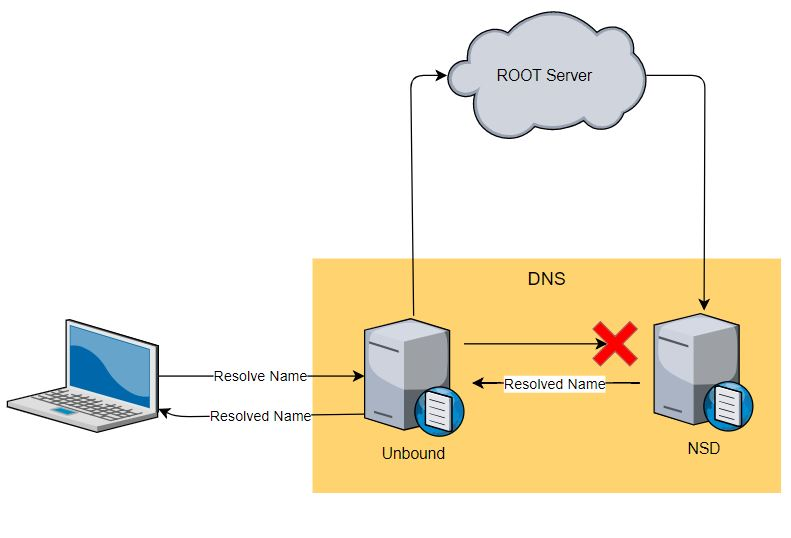
\includegraphics[width=\textwidth]{dns}

\noindent After the installation you will enter the domain management screen. Here you can add and remove domains. You can use multiple sub-domains of one domain, as it is configured with a wild-card and they will be resolved.

\subsubsection{Firewall}

In this step the UFW (uncomplicated firewall) will be installed and configured by the script. The firewall will be updated automatically each time you install or delete a module, so the corresponding ports can be opened or closed.

\subsubsection{Web server}

In this step the web server (apache2) and a reverse proxy (nginx) will be set up in two Docker containers. The following figure shows how the reverse proxy will interact with the web server. \newline

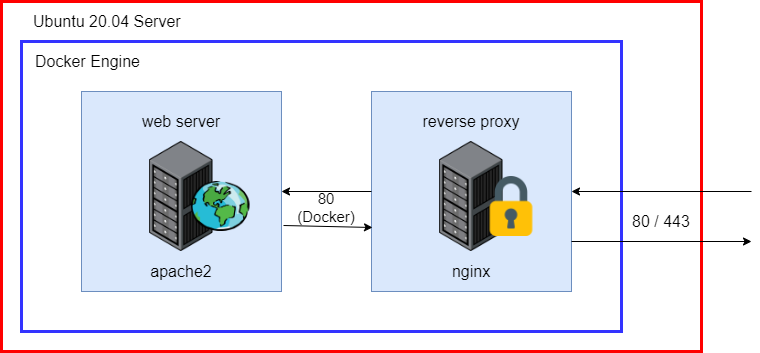
\includegraphics[width=\textwidth]{web} \newline


\noindent After selecting the installation for the web server, you will see the domain management screen. You can add and remove your domains here. \newline

\noindent IMPORTANT: Only use domains you own and which are registered on you. Otherwise it may be illegal or the challenge for your SSL certificates may fail. \newline

\noindent After the installation you can put your html or php files here: /srv/docker-web under the directory of your domain. They will be mapped into the container automatically and still remain in the directory even if the container is stopped. \newline

\noindent You can find the certificates for your websites in the following directory: /srv/docker-reverseproxy.

\subsubsection{MySQL}

A MySQL database and MySQL Adminer will be installed with this module. You will be able to reach the Adminer web interface on yourdomain.com/adminer. To connect the database to your website with msqli setting the host variable to the name of the container whis is mysql-db (\$host = 'mysql-db';). You can also reach your database from remote on port 3306.

\subsubsection{Mailu}

A Mailu mail server will be installed. You can reach the webmail on yourdomain.com/webmail and the admin panel on yourdomain.com/ui. You can only add one domain during the installation, but you will be able to add multiple domains and e-mail addresses later via the admin panel. For further information on Mailu please refer to \url{https://mailu.io/1.7/}.

\subsubsection{Jitsi}

IMPORTANT: The Jitsi server is a standalone server and can not be installed among side the web server, mail server or database. \newline 

\noindent Jitsi is a collection of free and open-source multiplatform voice (VoIP), videoconferencing and instant messaging applications. All the Jitsi components will be installed inside Docker containers. \newline

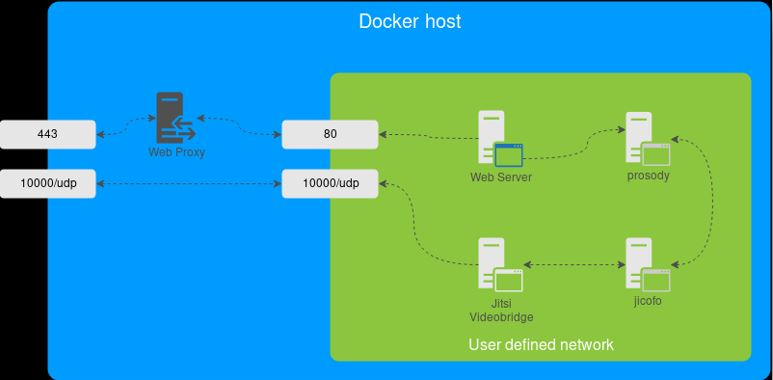
\includegraphics[width=\textwidth]{jitsi} \newline

\noindent After the installation the Jitsi web interface will be reachable on port 8443. \newline

\noindent For more information on Jitsi please go to \url{https://jitsi.org/}.

\subsubsection{Tor relay}

Tor is composed of a client, at least three middle nodes, and a public endpoint. In this script a middle relay will be set up automatically. You can choose a name for your relay and you have to provide an e-mail address. It is not possible to configure an exit relay with this script, as this may result in legal consequences and is only recommended for public organisations. After the installation you can check your relay here: \url{https://metrics.torproject.org/rs.html} (it may take a few hours until your relay is visible!).

\subsubsection{Snort}

Snort is an intrusion detection software that will log suspicious traffic such as scans or DDoS attempts. After the installation Snort will run in the background. You can find the logs in /var/log/snort/alert.

\noindent If snort should ever stop running (e.g. due to a reboot) you can just uninstall and install the snort moduel again or you can run "snort -i interface -l /var/log/snort -A fast -c /etc/snort/snort.conf -D" from your command line. \newline

\noindent For more information on Snort please go to: \url{https://www.snort.org/}.

\subsection{Remove Modules}

You can remove modules in the same way that you install them. Please take note that when removing Docker based modules you will have to run "update Docker" in the main menu afterwards for the containers to be removed.

\subsection{About Docker}

All Docker containers used in this script are set to restart automatically, should the host system be rebooted. You can check which containers are running by using the command "sudo docker container ls". If the containers should stop running just run the setup script again. If a container is stopped, everything inside will be deleted.For this reason the most important files and directories (such as websites and certificate) are mapped to the host system.

\end{document}